\chapter{Síntesis asimétrica}\label{ch:b3:asymmetric-synthesis}

La L-DOPA, el fármaco que alivia los síntomas de la enfermedad de Parkinson, fue en los
años setenta el primer compuesto fabricado industrialmente por \omterm{def:b3:asymmetric-synthesis:asymmetric-catalysis}{catálisis asimétrica}: unos pocos
gramos de un complejo quiral de rodio, disueltos con un precursor plano y aquiral
bajo hidrógeno, dieron un producto en el que un enantiómero superaba con mucho al
otro. Los dos enantiómeros de un fármaco pueden tener efectos completamente distintos,
porque los receptores y las \omterm{def:b3:complex-kinetics:enzyme}{enzimas} que encuentran son a su vez quirales. Este
capítulo mide la pureza enantiomérica, explica cómo un entorno quiral elige
entre dos caminos especulares y recorre las estrategias (\omterm{def:b3:asymmetric-synthesis:chiral-pool}{acervo quiral},
auxiliares, resoluciones, catalizadores metálicos y orgánicos) que producen enantiómeros
únicos.

\begin{recall}
El volumen del primer año definió la quiralidad, los enantiómeros, los diastereómeros, las mezclas
racémicas, la rotación específica, las reglas CIP y las reacciones estereoselectivas y
estereoespecíficas; el volumen del segundo año, la hidrogenación catalítica, la
epoxidación, la dihidroxilación, las iminas, las enaminas, los enolatos, la reacción aldólica,
la anelación de Robinson y la cromatografía. El \cref{ch:b3:rate-theories} dio la
\omterm{thm:b3:rate-theories:eyring}{ecuación de Eyring}; el \cref{ch:b3:homogeneous-catalysis}, el ciclo de Wilkinson, y
el \cref{ch:b3:point-groups}, el eje $C_2$.
\end{recall}

\begin{omfigure}
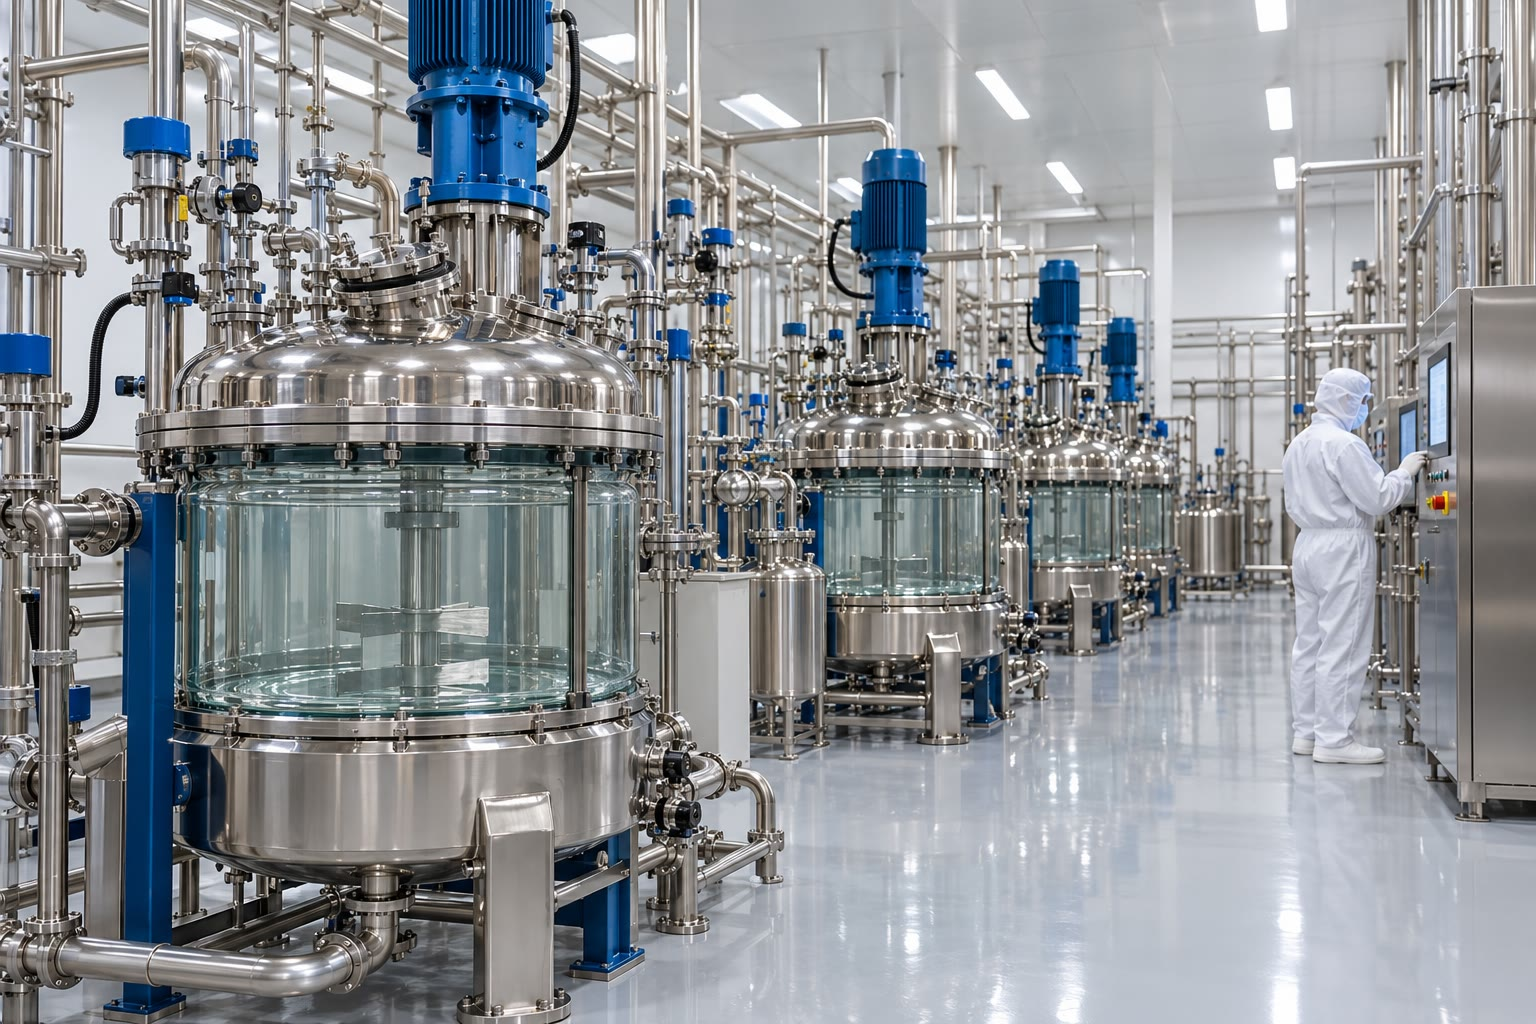
\includegraphics[width=0.58\linewidth]{images/book4/ai/b3-28-api-plant.jpg}

{\small Una nave de reactores esmaltados en una planta de fabricación de principios activos
farmacéuticos. Muchos de sus productos son enantiómeros únicos, obtenidos
por catálisis o por resolución y controlados por cromatografía quiral.}
\end{omfigure}

\section{Medir la pureza enantiomérica}

\begin{definition}[Exceso enantiomérico]\label{def:b3:asymmetric-synthesis:ee}
Para una mezcla de enantiómeros en cantidades $n_R \ge n_S$, el \emph{exceso
enantiomérico}\index{exceso enantiomerico@exceso enantiomérico} es $\mathrm{ee} = (n_R - n_S)/(n_R + n_S)$, y la \emph{relación enantiomérica}%
\index{relacion enantiomerica@relación enantiomérica}, $\mathrm{er} = n_R/n_S$; para los diastereómeros, el
\emph{exceso diastereomérico}\index{exceso diastereomerico@exceso diastereomérico}, ed, se define del
mismo modo. La \emph{pureza óptica}\index{pureza optica@pureza óptica} es la razón entre la
rotación específica de una muestra y la del enantiómero puro.
\end{definition}

\begin{proposition}[ee y er]\label{prop:b3:asymmetric-synthesis:ee-er}
$\mathrm{ee} = (\mathrm{er} - 1)/(\mathrm{er} + 1)$ y $\mathrm{er} = (1 + \mathrm{ee})/(1 - \mathrm{ee})$.
\end{proposition}

\begin{proof}
Se dividen el numerador y el denominador de $(n_R - n_S)/(n_R + n_S)$ por $n_S$; despejando er se obtiene la
segunda forma.
\end{proof}

Un ee del 90\,\% equivale a una er de 95\,:\,5, y un ee del 98\,\%, a una er de 99\,:\,1. La \omterm{def:b3:asymmetric-synthesis:ee}{pureza óptica}
solo es igual al ee si la rotación es proporcional a la composición; las impurezas, el
disolvente, los efectos de concentración y las pequeñas rotaciones de muchos compuestos la hacen
poco fiable, y el ee se mide separando los enantiómeros.

\begin{method}[El ee a partir de un cromatograma quiral]\label{met:b3:asymmetric-synthesis:ee-chromatogram}
\begin{enumerate}
  \item Inyectar primero el racémico, para identificar los dos picos y comprobar su
        separación (resolución hasta la línea de base) y la igualdad de sus áreas.
  \item Inyectar la muestra e integrar ambos picos.
  \item Los enantiómeros dan la misma respuesta en un detector aquiral, de modo que
        $\mathrm{ee} = (A_1 - A_2)/(A_1 + A_2)$; asignar los picos con un patrón enantiopuro.
\end{enumerate}
\end{method}

\begin{omfigure}
\begin{tikzpicture}
\begin{axis}[name=a, width=0.48\linewidth, height=5.4cm, xmin=0, xmax=20, ymin=0, ymax=1.0,
  axis lines=left, xlabel={$\Delta\Delta G^\ddagger$ / \unit{kJ.mol^{-1}}}, ylabel={ee},
  tick label style={font=\scriptsize}, label style={font=\small}]
\addplot[omDef, thick] table[x=ddg, y=eeA] {figdata/out/bachelor-3-er-ddg.dat};
\addplot[omMeth, thick] table[x=ddg, y=eeB] {figdata/out/bachelor-3-er-ddg.dat};
\addplot[omThm, thick] table[x=ddg, y=eeC] {figdata/out/bachelor-3-er-ddg.dat};
\node[font=\scriptsize, omDef, anchor=west] at (axis cs:10,0.55) {\qty{-78}{\celsius}};
\node[font=\scriptsize, omMeth, anchor=west] at (axis cs:10,0.43) {\qty{0}{\celsius}};
\node[font=\scriptsize, omThm, anchor=west] at (axis cs:10,0.31) {\qty{25}{\celsius} (curva inferior)};
\end{axis}
\begin{axis}[at={(a.east)}, anchor=west, xshift=1.4cm, width=0.48\linewidth, height=5.4cm,
  xmin=7.5, xmax=9.5, ymin=0, axis lines=left, ytick=\empty,
  xlabel={tiempo de retención / min}, ylabel={señal del detector},
  tick label style={font=\scriptsize}, label style={font=\small}]
\addplot[black, thick] table[x=t, y=y] {figdata/out/bachelor-3-er-ddg-b.dat};
\node[font=\scriptsize, anchor=south west] at (axis cs:8.3,250) {(\textit{R}): 97.5};
\node[font=\scriptsize, anchor=south] at (axis cs:9.1,20) {(\textit{S}): 2.5};
\end{axis}
\end{tikzpicture}

{\small Izquierda: \omterm{def:b3:asymmetric-synthesis:ee}{exceso enantiomérico} en función de la diferencia de \omterm{def:b3:rate-theories:activation}{energía de Gibbs de
activación} de los dos caminos en competencia, a tres temperaturas: la misma
$\Delta\Delta G^\ddagger$ da un ee mayor a baja temperatura. Derecha: un cromatograma de HPLC quiral,
con áreas de pico de 97.5 y 2.5 (modelo): ee del 95\,\%.}
\end{omfigure}

La RMN solo distingue los enantiómeros en un entorno quiral: un agente de solvatación
quiral forma complejos diastereoméricos de vida corta cuyas señales difieren, y un
alcohol o una amina quirales convertidos en sus dos ésteres diastereoméricos con el
ácido de Mosher muestran la configuración a partir del patrón de las diferencias de desplazamiento.

\begin{method}[La configuración a partir de los ésteres de Mosher, a grandes rasgos]\label{met:b3:asymmetric-synthesis:mosher}
\begin{enumerate}
  \item Preparar los dos ésteres de MTPA, (\textit{R}) y (\textit{S}), del alcohol.
  \item Registrar sus espectros de protón y calcular $\Delta\delta = \delta_S - \delta_R$ para los protones de cada
        lado del carbono carbinólico.
  \item En la conformación preferida, el anillo fenilo del ácido apantalla un lado:
        los protones con $\Delta\delta > 0$ están a un lado, y los de $\Delta\delta < 0$, al otro, lo que
        sitúa los dos sustituyentes y da la configuración.
\end{enumerate}
\end{method}

\section{Topicidad y adiciones estereoselectivas}

\begin{definition}[Reacciones estereoselectivas]\label{def:b3:asymmetric-synthesis:selective}
Una \emph{reacción enantioselectiva}\index{reaccion enantioselectiva@reacción enantioselectiva} forma un
enantiómero de un producto en exceso respecto del otro; una \emph{reacción
diastereoselectiva}\index{reaccion diastereoselectiva@reacción diastereoselectiva} forma un diastereómero en exceso.
\end{definition}

\begin{definition}[Topicidad]\label{def:b3:asymmetric-synthesis:topicity}
Dos grupos de una molécula son \emph{homotópicos}\index{homotopico@homotópico} cuando los intercambia
una rotación de la molécula (sustituir cualquiera de ellos da el mismo compuesto);
\emph{enantiotópicos}\index{enantiotopico@enantiotópico}, cuando solo los intercambia una reflexión
(sustituir uno u otro da enantiómeros), y
\emph{diastereotópicos}\index{diastereotopico@diastereotópico}, cuando ninguna \omterm{def:b3:point-groups:operation}{operación de simetría} los
intercambia (sustituir uno u otro da diastereómeros).
\end{definition}

Los dos hidrógenos de un grupo $\ce{CH2}$ contiguo a un estereocentro son \omterm{def:b3:asymmetric-synthesis:topicity}{diastereotópicos}:
tienen desplazamientos químicos distintos y se acoplan entre sí, por lo que un grupo así
suele dar dos señales en RMN.

\begin{definition}[Caras proquirales]\label{def:b3:asymmetric-synthesis:faces}
Un carbono trigonal con tres sustituyentes distintos es \emph{proquiral}\index{proquiral}:
la adición de un cuarto grupo, distinto, crea un estereocentro. Su cara vista con
los tres sustituyentes, por orden de prioridad CIP decreciente, recorridos en el sentido de las agujas del reloj es la
\emph{cara Re}\index{cara Re}; en el sentido contrario, la \emph{cara Si}\index{cara Si}.
\end{definition}

\begin{omfigure}
\begin{tikzpicture}[font=\small, >=Stealth]
  \coordinate (c) at (0,0);
  \draw[thick, double, double distance=1.6pt] (c) -- (90:1.1) node[above] {O (1)};
  \draw[thick] (c) -- (210:1.1) node[below left] {$\ce{C6H5}$ (2)};
  \draw[thick] (c) -- (330:1.1) node[below right] {$\ce{CH3}$ (3)};
  \fill (c) circle (1.6pt);
  \draw[->, thick, omThm] (70:0.6) arc[start angle=70, end angle=200, radius=0.6];
  \node[font=\scriptsize, omThm, align=center] at (-1.9,0.75) {1 $\to$ 2 $\to$ 3\\ en sentido antihorario:\\ cara \textit{Si}};
  \node[font=\scriptsize, align=left, anchor=west] at (2.6,0.4) {cara hacia el lector: \textit{Si}\\ cara detrás de la página: \textit{Re}};
  \node[font=\scriptsize, align=left, anchor=west] at (2.6,-0.5) {el hidruro añadido por la cara \textit{Re}\\ da el (\textit{S})-1-feniletanol};
\end{tikzpicture}

{\small Las caras de la acetofenona. Vistos desde delante, los sustituyentes del
carbono carbonílico en orden CIP (O, fenilo, metilo) se suceden en sentido antihorario: la cara
delantera es \textit{Si}, y la trasera, \textit{Re}.}
\end{omfigure}

\begin{method}[Asignar las caras Re y Si]\label{met:b3:asymmetric-synthesis:re-si}
\begin{enumerate}
  \item Clasificar los tres sustituyentes del átomo trigonal según las reglas CIP (un
        doble enlace cuenta dos veces su compañero).
  \item Mirar la cara de interés, con el plano trigonal en el plano de la página.
  \item Sentido horario 1 $\to$ 2 $\to$ 3: \textit{Re}; sentido antihorario: \textit{Si}.
  \item Para nombrar el producto, añadir el nuevo grupo hacia el observador y aplicar las
        reglas CIP al nuevo estereocentro; el ataque por la \omterm{def:b3:asymmetric-synthesis:faces}{cara Re} no siempre da \textit{R}.
\end{enumerate}
\end{method}

\begin{definition}[Modelo de Felkin--Anh y control por quelación]\label{def:b3:asymmetric-synthesis:felkin}
El \emph{modelo de Felkin--Anh}\index{modelo de Felkin--Anh} predice el diastereómero
mayoritario de una adición nucleófila a un grupo carbonilo contiguo a un
estereocentro: el grupo más grande de ese centro se sitúa perpendicular al
plano del carbonilo, y el nucleófilo se aproxima en anti respecto de él, junto al grupo
más pequeño, siguiendo la trayectoria de Bürgi--Dunitz. En el \emph{control
por quelación}\index{control por quelacion@control por quelación}, un ion metálico unido a la vez al oxígeno del carbonilo
y a un grupo dador del estereocentro bloquea la conformación, y el
nucleófilo se adiciona por la cara menos impedida del anillo quelato.
\end{definition}

\begin{proposition}[Selectividad de Felkin--Anh]\label{prop:b3:asymmetric-synthesis:felkin}
Para un aldehído o una cetona $\alpha$-quirales sin grupo quelante, el producto
mayoritario es el que predice el \omterm{def:b3:asymmetric-synthesis:felkin}{modelo de Felkin--Anh} (un modelo empírico,
respaldado por el cálculo). \admitted
\end{proposition}

\begin{omfigure}
\begin{tikzpicture}[font=\small, >=Stealth]
  \foreach \a/\lab in {90/L, 330/M, 210/S} {
    \draw[line width=0.8pt] (\a:0.55) -- (\a:1.1) node[pos=1.3] {\lab};
  }
  \fill[white] (0,0) circle (0.55);
  \draw[line width=0.8pt] (0,0) circle (0.55);
  \draw[line width=0.8pt, double, double distance=1.4pt] (0,0) -- (0:1.1) node[right] {O};
  \draw[line width=0.8pt] (0,0) -- (180:1.1) node[left] {R};
  \draw[->, very thick, omThm] (250:2.2) -- (250:0.25);
  \node[omThm, anchor=north] at (250:2.25) {Nu$^-$};
  \node[font=\scriptsize, align=left, anchor=west] at (1.7,-1.0) {Nu$^-$ entra en anti respecto de L,\\ junto a S, a unos 107°\\ del enlace C=O};
\end{tikzpicture}

{\small \omterm{def:b3:asymmetric-synthesis:felkin}{Modelo de Felkin--Anh}, visto a lo largo del enlace que va del carbono carbonílico (delante,
enlaces con O y con R) al estereocentro (círculo trasero, grupos L, M y S). El
grupo grande es perpendicular al plano del carbonilo; el nucleófilo llega por
el lado opuesto, cerca del grupo pequeño y lejos del oxígeno.}
\end{omfigure}

\section{Estrategias}

\begin{definition}[Acervo quiral]\label{def:b3:asymmetric-synthesis:chiral-pool}
El \emph{acervo quiral}\index{acervo quiral} es el conjunto de compuestos naturales baratos
y enantiopuros (aminoácidos, azúcares, terpenos, hidroxiácidos) usados como
materiales de partida, cuyos estereocentros se trasladan a la molécula objetivo.
\end{definition}

\begin{definition}[Auxiliar quiral]\label{def:b3:asymmetric-synthesis:auxiliary}
Un \emph{auxiliar quiral}\index{auxiliar quiral} es un grupo enantiopuro
unido temporalmente a un sustrato para controlar la estereoquímica de una
reacción, que después se elimina y se recupera.
\end{definition}

En las alquilaciones de Evans, se acila una oxazolidinona preparada a partir de un aminoácido;
el enolato de litio o de sodio, quelado por el grupo carbonilo del auxiliar, es
atacado por un haluro de alquilo por la cara opuesta al sustituyente del auxiliar,
lo que da un solo diastereómero, a menudo con un ed superior al 95\,\%; la hidrólisis libera después el
ácido quiral y el auxiliar.

\begin{definition}[Resoluciones]\label{def:b3:asymmetric-synthesis:resolution}
La \emph{resolución de un racémico}\index{resolucion de un racemico@resolución de un racémico} es su
separación en enantiómeros, clásicamente por cristalización de sales diastereoméricas
con un ácido o una base enantiopuros. En una \emph{resolución cinética}\index{resolucion cinetica@resolución cinética},
los dos enantiómeros reaccionan a velocidades distintas con un reactivo o un
catalizador quirales, con una selectividad $s = k_{\text{rápida}}/k_{\text{lenta}}$. En una \emph{resolución
cinética dinámica}\index{resolucion cinetica dinamica@resolución cinética dinámica}, los enantiómeros del sustrato
se interconvierten deprisa mientras uno de ellos reacciona.
\end{definition}

\begin{theorem}[Ecuación de Kagan]\label{thm:b3:asymmetric-synthesis:kagan}
En una \omterm{def:b3:asymmetric-synthesis:resolution}{resolución cinética} de un racémico mediante reacciones de primer orden de selectividad $s$,
la conversión $c$ y el ee del sustrato restante están relacionados por
\[
  s = \frac{\ln[(1 - c)(1 - \mathrm{ee})]}{\ln[(1 - c)(1 + \mathrm{ee})]}.
\]
\end{theorem}

\begin{proof}
Cada enantiómero decae exponencialmente: las fracciones restantes son $f_1 = \eu^{-k_{\text{rápida}}t}$ y
$f_2 = \eu^{-k_{\text{lenta}}t}$, luego $\ln f_1 = s\ln f_2$. Partiendo de cantidades iguales, $1 - c = (f_1 + f_2)/2$ y
$\mathrm{ee} = (f_2 - f_1)/(f_1 + f_2)$. Entonces $(1 - c)(1 - \mathrm{ee}) = \tfrac12(f_1 + f_2)\cdot 2f_1/(f_1 + f_2) = f_1$ y, del mismo modo,
$(1 - c)(1 + \mathrm{ee}) = f_2$. Por tanto, $s = \ln f_1/\ln f_2$ es el cociente enunciado.
\end{proof}

\begin{omfigure}
\begin{tikzpicture}
\begin{axis}[width=0.62\linewidth, height=5.6cm, xmin=0, xmax=1, ymin=0, ymax=1.02,
  axis lines=left, xlabel={conversión $c$}, ylabel={ee},
  tick label style={font=\scriptsize}, label style={font=\small},
  legend style={font=\scriptsize, draw=none, at={(1.04,0.5)}, anchor=west}, legend cell align=left]
\addplot[color=omThm, thick] table[x=c, y=eesm] {figdata/out/bachelor-3-kinetic-resolution-s2.dat};
\addlegendentry{$s = 2$}
\addplot[color=omMeth, thick] table[x=c, y=eesm] {figdata/out/bachelor-3-kinetic-resolution-s10.dat};
\addlegendentry{$s = 10$}
\addplot[color=omDef, thick] table[x=c, y=eesm] {figdata/out/bachelor-3-kinetic-resolution-s50.dat};
\addlegendentry{$s = 50$}
\addplot[color=omThm, thick, dashed] table[x=c, y=eep] {figdata/out/bachelor-3-kinetic-resolution-s2.dat};
\addplot[color=omMeth, thick, dashed] table[x=c, y=eep] {figdata/out/bachelor-3-kinetic-resolution-s10.dat};
\addplot[color=omDef, thick, dashed] table[x=c, y=eep] {figdata/out/bachelor-3-kinetic-resolution-s50.dat};
\end{axis}
\end{tikzpicture}

{\small \omterm{def:b3:asymmetric-synthesis:resolution}{Resolución cinética}: ee del sustrato restante (trazo continuo) y del
producto (trazo discontinuo) en función de la conversión, para tres selectividades. El sustrato
siempre puede hacerse enantiopuro avanzando lo suficiente, a costa del rendimiento; el
producto es más puro a baja conversión.}
\end{omfigure}

\begin{proposition}[Resolución cinética dinámica]\label{prop:b3:asymmetric-synthesis:dkr}
Si los enantiómeros del sustrato se interconvierten mucho más deprisa de lo que reacciona cualquiera de ellos,
todo el racémico puede convertirse en un solo enantiómero del producto, con un ee fijado por $s$:
$\mathrm{er} = s$.
\end{proposition}

\begin{proof}
La racemización rápida mantiene los dos enantiómeros del sustrato en cantidades iguales en todo
momento. Los productos se forman entonces a velocidades en la razón $k_{\text{rápida}}[\mathrm A] : k_{\text{lenta}}[\mathrm A] = s$, y nada
detiene la reacción antes de que se consuma todo el sustrato, sobre todo a través del enantiómero rápido:
el rendimiento puede alcanzar el 100\,\% con $\mathrm{er} = s$.
\end{proof}

\begin{method}[Elegir una estrategia]\label{met:b3:asymmetric-synthesis:strategy}
\begin{enumerate}
  \item Si los estereocentros de la molécula objetivo existen en un compuesto natural barato, partir
        del \omterm{def:b3:asymmetric-synthesis:chiral-pool}{acervo quiral}.
  \item Para una síntesis puntual, o para fijar de forma fiable un centro contiguo a un grupo
        carbonilo, usar un auxiliar, a costa de dos etapas adicionales.
  \item Si el racémico es barato y el enantiómero no deseado puede reciclarse o
        racemizarse, resolverlo (de forma clásica, cinética o dinámica).
  \item A gran escala, buscar un catalizador asimétrico: un estereocentro creado
        por ciclo catalítico, sin residuos quirales estequiométricos.
\end{enumerate}
\end{method}

\section{Catálisis asimétrica con metales}

\begin{definition}[Catálisis asimétrica]\label{def:b3:asymmetric-synthesis:asymmetric-catalysis}
La \emph{catálisis asimétrica}\index{catalisis asimetrica@catálisis asimétrica} es la síntesis enantioselectiva
con un catalizador quiral usado en pequeña cantidad; en los catalizadores metálicos, la
quiralidad procede normalmente de un \emph{ligando quiral}\index{ligando quiral}.
\end{definition}

\begin{theorem}[La selectividad a partir de la energía]\label{thm:b3:asymmetric-synthesis:er-ddg}
Si dos productos enantioméricos se forman a través de estados de transición diastereoméricos
con factores preexponenciales iguales, de forma irreversible y bajo control cinético,
$\mathrm{er} = \exp(\Delta\Delta G^\ddagger/RT)$, donde $\Delta\Delta G^\ddagger$ es la diferencia de sus \omterm{def:b3:rate-theories:activation}{energías de Gibbs de
activación}.
\end{theorem}

\begin{proof}
Según la \omterm{thm:b3:rate-theories:eyring}{ecuación de Eyring} (\cref{ch:b3:rate-theories}),
$k_i = (k_BT/h)\eu^{-\Delta G_i^\ddagger/RT}$; ambos productos se forman a partir de los mismos reactivos, de modo que en cada instante
sus velocidades están en la razón $k_1/k_2 = \eu^{(\Delta G_2^\ddagger - \Delta G_1^\ddagger)/RT}$, y también lo están las cantidades formadas.
\end{proof}

A \qty{25}{\celsius}, un ee del 99\,\% (er de 199) exige $\Delta\Delta G^\ddagger = RT\ln 199 = \qty{13.1}{kJ/mol}$, del orden de la energía de un
solo enlace de hidrógeno; a \qty{-78}{\celsius} bastan \qty{8.6}{kJ/mol}.

\begin{proposition}[Ligandos de simetría $C_2$]\label{prop:b3:asymmetric-synthesis:c2}
Un \omterm{def:b3:asymmetric-synthesis:asymmetric-catalysis}{ligando quiral} de simetría $C_2$ reduce a la mitad el número de estados de transición diastereoméricos
que hay que comparar, ya que las dos posiciones de coordinación que deja libres son
equivalentes.
\end{proposition}

\begin{proof}
La rotación $C_2$ del catalizador transforma una posición libre en la otra y deja el
catalizador inalterado; todo estado de transición en una posición es, por tanto, idéntico al
estado girado en la otra. Solo hay que comparar los modos de unión en una posición (cara del sustrato,
orientación).
\end{proof}

Knowles usó monofosfinas quirales y después la difosfina de simetría $C_2$ DIPAMP, con rodio, para
hidrogenar una enamida al aminoácido protegido de la L-DOPA; el BINAP de Noyori,
con rutenio, hidrogena cetonas y alquenos funcionalizados y,
combinado con una diamina quiral, cetonas sencillas con ee muy altos. En la
hidrogenación de enamidas con rodio, el producto mayoritario procede del complejo catalizador--sustrato
minoritario y menos estable, que reacciona mucho más deprisa con el hidrógeno: la
selectividad se fija en los estados de transición, no por las \omterm{def:b3:partition-functions:boltzmann}{poblaciones} de los
intermedios (el principio de Curtin--Hammett).

\begin{definition}[Epoxidación de Sharpless]\label{def:b3:asymmetric-synthesis:sharpless}
La \emph{epoxidación de Sharpless}\index{epoxidacion de Sharpless@epoxidación de Sharpless} es la
epoxidación enantioselectiva de alcoholes alílicos con hidroperóxido de \textit{terc}-butilo,
catalizada por isopropóxido de titanio(IV) con un tartrato de dietilo enantiopuro; el
alcohol se une al titanio, que entrega el oxígeno a una cara del
alqueno, elegida por el tartrato.
\end{definition}

\begin{omfigure}
\begin{tikzpicture}[font=\small, >=Stealth]
  \draw[black!50] (-2.3,-1.55) rectangle (2.5,1.55);
  % C3 (top) = C2 (bottom); C2 carries R1 (left) and CH2OH (lower right),
  % C3 carries R2 (left) and R3 (right)
  \coordinate (c3) at (0,0.45); \coordinate (c2) at (0,-0.45);
  \draw[thick, double, double distance=1.6pt] (c3) -- (c2);
  \draw[thick] (c3) -- (-0.9,0.95) node[above left, inner sep=1pt] {R$^2$};
  \draw[thick] (c3) -- (0.9,0.95) node[above right, inner sep=1pt] {R$^3$};
  \draw[thick] (c2) -- (-0.9,-0.95) node[below left, inner sep=1pt] {R$^1$};
  \draw[thick] (c2) -- (0.9,-0.95) node[below right, inner sep=1pt] {$\ce{CH2OH}$};
  \draw[->, very thick, omDef] (0.35,2.5) -- (0.2,0.1) node[pos=0, above, align=center, font=\scriptsize] {tartrato de dietilo D-($-$):\\ O por la cara superior};
  \draw[->, very thick, omThm] (0.35,-2.6) -- (0.2,-0.1) node[pos=0, below, align=center, font=\scriptsize] {tartrato de dietilo L-($+$):\\ O por la cara inferior};
\end{tikzpicture}

{\small La regla mnemotécnica de Sharpless. Con el alcohol alílico dibujado en el plano y el
grupo $\ce{CH2OH}$ abajo a la derecha, el tartrato de dietilo L-($+$) entrega el oxígeno por
debajo del plano, y el tartrato de dietilo D-($-$), por encima, sean cuales sean los
sustituyentes $\mathrm R^1$ a $\mathrm R^3$.}
\end{omfigure}

La misma idea, un metal sujeto en un bolsillo quiral por un ligando natural barato, da la
dihidroxilación asimétrica de Sharpless de los alquenos con osmio y ligandos alcaloides de la
quina. Cuando el ligando no es enantiopuro, el ee del producto
no tiene por qué ser proporcional al del ligando: los agregados de dos ligandos, con
actividades distintas para los pares homoquirales y heteroquirales, dan efectos
no lineales, a veces amplificaciones útiles.

\section{Organocatálisis}

\begin{definition}[Organocatálisis]\label{def:b3:asymmetric-synthesis:organocatalysis}
La \emph{organocatálisis}\index{organocatalisis@organocatálisis} es la catálisis por pequeñas moléculas
orgánicas sin metales. En la \emph{catálisis por enamina}\index{catalisis por enamina@catálisis por enamina}, una
amina secundaria convierte una cetona o un aldehído en una enamina nucleófila; en la
\emph{catálisis por iminio}\index{catalisis por iminio@catálisis por iminio}, convierte un aldehído $\alpha,\beta$-insaturado
en un ion iminio electrófilo con una LUMO rebajada.
\end{definition}

\begin{omfigure}
\begin{tikzpicture}[font=\small]
  % proline-derived enamine and the aldehyde held by the carboxylic acid
  \coordinate (n) at (0,0.7); \coordinate (r2) at (0.67,0.22); \coordinate (r3) at (0.41,-0.57);
  \coordinate (r4) at (-0.41,-0.57); \coordinate (r5) at (-0.67,0.22);
  \draw[thick] (n) -- (r2) -- (r3) -- (r4) -- (r5) -- (n);
  \node[fill=white, inner sep=0.6pt] at (n) {N};
  \coordinate (ca) at (0,1.45); \coordinate (cb) at (0.72,1.85);
  \draw[thick] (0,0.88) -- (ca);
  \draw[thick] (ca) -- (-0.62,1.85) node[left, inner sep=1pt] {$\ce{CH3}$};
  \draw[thick, double, double distance=1.5pt] (ca) -- (cb);
  \coordinate (cacid) at (1.45,0.45);
  \draw[thick] (r2) -- (cacid);
  \draw[thick, double, double distance=1.5pt] (cacid) -- (1.75,-0.15) node[below, inner sep=1pt] {O};
  \draw[thick] (cacid) -- (2.05,0.9) node[right, inner sep=1pt] (oh) {O--H};
  \node (cald) at (1.55,2.55) {C};
  \draw[thick, double, double distance=1.5pt] (cald) -- (2.35,2.15) node[right, inner sep=1pt] (oald) {O};
  \draw[thick] (cald) -- (1.3,3.15) node[above, inner sep=1pt] {R};
  \draw[omThm, thick, densely dashed] (cb) -- (cald);
  \draw[omMeth, thick, dotted] (2.45,1.05) -- (2.5,2.0);
  \node[font=\scriptsize, omThm, anchor=east] at (1.05,2.35) {se forma C--C};
  \node[font=\scriptsize, omMeth, anchor=west] at (2.6,1.55) {enlace de H};
\end{tikzpicture}

{\small La reacción aldólica catalizada por prolina, estado de transición esquemático: la
enamina formada a partir de la acetona y del nitrógeno de la pirrolidina ataca el aldehído,
cuyo oxígeno está sujeto por un enlace de hidrógeno al ácido carboxílico del catalizador;
ese enlace fija qué cara del aldehído es atacada.}
\end{omfigure}

La prolina, un aminoácido barato, cataliza reacciones aldólicas intramoleculares de
tricetonas con ee altos (las cetonas de Hajos--Parrish y de Wieland--Miescher, usadas
desde los años setenta en síntesis de esteroides) y, como se demostró en 2000, reacciones
aldólicas intermoleculares de la acetona con aldehídos. Las imidazolidinonas quirales actúan a través de
iones iminio en reacciones de Diels--Alder y en adiciones conjugadas; los
ácidos fosfóricos quirales, ácidos de Brønsted fuertes con un bolsillo quiral, activan las iminas
por protonación. Los organocatalizadores son estables al aire y al agua y no dejan metal
en el producto.

\begin{inthelab}[Un análisis por HPLC quiral]
Una columna quiral, de sílice recubierta con un derivado de celulosa o de amilosa, se
equilibra con una mezcla hexano--isopropanol. Se inyecta primero el racémico
y se ajusta la proporción de disolventes hasta que los dos picos estén separados hasta la línea de base; después
se inyecta la muestra, disuelta en el eluyente a aproximadamente un miligramo por mililitro,
y se integran los picos a una longitud de onda a la que ambos absorben.
\end{inthelab}

\begin{safety}{\ghs[0.6cm]{GHS02}\ghs[0.6cm]{GHS05}\ghs[0.6cm]{GHS06}\ghs[0.6cm]{GHS08}\ghs[0.6cm]{GHS09}}
% ledger: ghs4:TBHP, ghs4:TiOiPr4
Hidroperóxido de \textit{terc}-butilo: inflamable, autorreactivo al calentarlo, tóxico en contacto con la
piel, corrosivo, sensibilizante, se sospecha que provoca defectos genéticos; se usa
en disolución, conservado en frío, nunca concentrado, y el peróxido en exceso se destruye
antes del tratamiento. Isopropóxido de titanio(IV): inflamable, irritante, se descompone con la
humedad.
\end{safety}

\begin{history}[Dos premios para la catálisis asimétrica]
William Knowles, Ryoji Noyori y Barry Sharpless compartieron el Premio Nobel
de Química de 2001 por las hidrogenaciones y oxidaciones catalizadas quiralmente. Benjamin List
y David MacMillan, que habían demostrado en 2000 que pequeñas moléculas orgánicas podían
catalizar \omterm{def:b3:asymmetric-synthesis:selective}{reacciones enantioselectivas} de forma tan general como los complejos metálicos, recibieron
el premio de 2021.
\end{history}

\section{Ejercicios}

\begin{exercise}[$\star$]\label{exo:b3:asymmetric-synthesis:1}
Conviértase: un ee del 80\,\% en er; una er de 99\,:\,1 en ee; un ee del 50\,\% en el porcentaje de cada
enantiómero.
\end{exercise}

\begin{exercise}[$\star$]\label{exo:b3:asymmetric-synthesis:2}
Un cromatograma de HPLC quiral muestra picos de áreas 1840 y 60 para los dos enantiómeros.
Calcúlese el ee.
\end{exercise}

\begin{exercise}[$\star$]\label{exo:b3:asymmetric-synthesis:3}
Asígnense las \omterm{def:b3:asymmetric-synthesis:faces}{caras Re} y Si del carbono carbonílico del propanal, y nómbrese el alcohol
formado por adición de un nucleófilo metilo por la \omterm{def:b3:asymmetric-synthesis:faces}{cara Re}.
\end{exercise}

\begin{exercise}[$\star$]\label{exo:b3:asymmetric-synthesis:4}
¿Son los dos protones metilénicos del etanol \omterm{def:b3:asymmetric-synthesis:topicity}{homotópicos}, \omterm{def:b3:asymmetric-synthesis:topicity}{enantiotópicos} o \omterm{def:b3:asymmetric-synthesis:topicity}{diastereotópicos}?
¿Y los del grupo $\ce{CH2}$ del 2-butanol?
\end{exercise}

\begin{exercise}[$\star\star$]\label{exo:b3:asymmetric-synthesis:5}
Calcúlense la $\Delta\Delta G^\ddagger$ necesaria para un ee del 99\,\% a \qty{25}{\celsius} y a \qty{-78}{\celsius}, y el ee que da a \qty{-78}{\celsius}
un catalizador que da un ee del 80\,\% a \qty{25}{\celsius} (con la misma $\Delta\Delta G^\ddagger$).
\end{exercise}

\begin{exercise}[$\star\star$]\label{exo:b3:asymmetric-synthesis:6}
Una muestra de una amina tiene $[\alpha]_D = -12.0$ en unas condiciones en las que el enantiómero (\textit{S})
puro tiene $-15.0$ (datos del ejercicio). Dense su \omterm{def:b3:asymmetric-synthesis:ee}{pureza óptica} y los
porcentajes de los enantiómeros, suponiendo la rotación proporcional a la composición.
¿Por qué esta medida es menos fiable que la cromatografía?
\end{exercise}

\begin{exercise}[$\star\star$]\label{exo:b3:asymmetric-synthesis:7}
En una acetilación de un alcohol racémico catalizada por una lipasa, el alcohol restante
tiene un ee del 90\,\% a una conversión del 60\,\%. Calcúlese $s$.
\end{exercise}

\begin{exercise}[$\star\star$]\label{exo:b3:asymmetric-synthesis:8}
Predígase el epóxido formado a partir del (\textit{E})-hex-2-en-1-ol con el tartrato de dietilo L-($+$), y con el
tartrato de dietilo D-($-$).
\end{exercise}

\begin{exercise}[$\star\star$]\label{exo:b3:asymmetric-synthesis:9}
El (\textit{S})-2-fenilpropanal se trata con bromuro de metilmagnesio. Úsese el \omterm{def:b3:asymmetric-synthesis:felkin}{modelo de
Felkin--Anh} para predecir el diastereómero mayoritario.
\end{exercise}

\begin{exercise}[$\star\star\star$]\label{exo:b3:asymmetric-synthesis:10}
Demuéstrese que en una \omterm{def:b3:asymmetric-synthesis:resolution}{resolución cinética} el ee del producto tiende a $(s - 1)/(s + 1)$ a baja
conversión, y calcúlese para $s = 20$. ¿Por qué una \omterm{def:b3:asymmetric-synthesis:resolution}{resolución cinética} es mejor para purificar
el sustrato que para obtener el producto?
\end{exercise}

\begin{exercise}[$\star\star\star$]\label{exo:b3:asymmetric-synthesis:11}
Una cetona con un estereocentro racemizable contiguo al grupo carbonilo se reduce con
una \omterm{def:b3:complex-kinetics:enzyme}{enzima} con $s = 99$, mientras que la racemización es rápida. ¿Qué rendimiento y qué ee pueden
alcanzarse? Compárese con la misma \omterm{def:b3:complex-kinetics:enzyme}{enzima} sin racemización, detenida al 50\,\% de
conversión.
\end{exercise}

\begin{exercise}[$\star\star\star$]\label{exo:b3:asymmetric-synthesis:12}
Explíquese con el principio de Curtin--Hammett cómo el complejo catalizador--sustrato minoritario
puede dar el producto mayoritario, usando dos complejos en equilibrio
($K = 10$ a favor de A) que reaccionan con $k_B/k_A = 600$.
\end{exercise}

\section{Problema: la ruta de la L-DOPA}

\begin{problem}[{Problema de fin de semana --- la ruta de la L-DOPA: la enamida proquiral y sus
caras, la energía que hay detrás de un ee del 95\,\%, la purificación por cristalización y lo que
habría necesitado una resolución cinética}]
\label{pb:b3:asymmetric-synthesis:1}
% ledger: const:R
Datos del problema: la hidrogenación catalizada por rodio del precursor
enamida a \qty{25}{\celsius} da el (\textit{S})-aminoácido protegido con un ee del 95\,\%. El producto
bruto, 100 g, se recristaliza: las aguas madres retienen todo el enantiómero
minoritario y 5.0 g del mayoritario.

\medskip\noindent\textbf{Parte I --- El sustrato.}
\begin{enumerate}
  \item ¿Por qué es \omterm{def:b3:asymmetric-synthesis:faces}{proquiral} la enamida? ¿Qué carbono se convierte en estereocentro?
  \item ¿Qué daría un catalizador aquiral?
  \item ¿Por qué importa al catalizador el grupo amida del alqueno?
  \item ¿Qué hace la difosfina quiral?
  \item ¿Se forma el producto mayoritario a partir del complejo catalizador--sustrato más
        estable?
  \item ¿Por qué el hidrógeno se añade por una sola cara en cada complejo?
\end{enumerate}

\medskip\noindent\textbf{Parte II --- Energía.}
\begin{enumerate}[resume]
  \item Dese la er correspondiente a un ee del 95\,\%.
  \item Calcúlese $\Delta\Delta G^\ddagger$ a \qty{25}{\celsius}.
  \item ¿Qué ee daría la misma $\Delta\Delta G^\ddagger$ a \qty{-78}{\celsius}?
  \item ¿Qué ee daría a \qty{25}{\celsius} una $\Delta\Delta G^\ddagger$ mayor en \qty{2}{kJ/mol}?
  \item Compárense \qty{9}{kJ/mol} con la energía de un enlace de hidrógeno, y coméntese.
  \item ¿Por qué no se lleva a cabo simplemente la reacción a menor temperatura?
\end{enumerate}

\medskip\noindent\textbf{Parte III --- Cristalización.}
\begin{enumerate}[resume]
  \item Calcúlense las masas de los dos enantiómeros en el producto bruto.
  \item Calcúlense la masa y el ee de los cristales.
  \item Calcúlese el rendimiento de la cristalización.
  \item ¿Por qué la cristalización puede elevar el ee de una muestra pero nunca crearlo a partir de un
        racémico (para un compuesto que cristaliza como compuesto racémico)?
  \item ¿Cómo se comprueba el ee final?
\end{enumerate}

\medskip\noindent\textbf{Parte IV --- Una \omterm{def:b3:asymmetric-synthesis:resolution}{resolución cinética} en su lugar.}
\begin{enumerate}[resume]
  \item ¿Cuál es el rendimiento máximo de un enantiómero en una \omterm{def:b3:asymmetric-synthesis:resolution}{resolución cinética} simple?
  \item Calcúlese el $s$ necesario para un ee del 95\,\% del sustrato restante a una conversión del 55\,\%.
  \item ¿Qué rendimiento de ese sustrato se obtiene?
  \item ¿Cómo cambiaría el rendimiento una \omterm{def:b3:asymmetric-synthesis:resolution}{resolución cinética dinámica}?
  \item ¿Por qué la hidrogenación asimétrica fue la mejor elección industrial?
  \item ¿Por qué hay que eliminar el rodio del fármaco, y cómo se mide?
  \item Enúnciese el resultado: la $\Delta\Delta G^\ddagger$ para un ee del 95\,\% a \qty{25}{\celsius}.
\end{enumerate}
\end{problem}
